

This chapter gives routines and tools for computing and using scalar and vector wave functions in free-space spherical coordinates. The wave functions represent the frequency-domain multipoles of the field, which together give the multipole expansion of a field. While the wave functions themselves are not always used, the coefficients of the expansions are quite useful. The expansion coefficients can be quickly manipulated by rotation and translation addition theorems to transform the fields in different reference frames (see Chapters \ref{chap:rotation} and \ref{chap:translation}). This chapter provides codes for spherical wave functions and serves as a quick reference for certain properties and derivations. 

\section{Indexing}

Spherical harmonics and spherical wave functions are defined by the degree and order of the underlying associated Legendre polynomials, $(l,m)$. It is convenient to store and access harmonics using a linear index. For vector wave functions, where the harmonics range from $l = 1,...,L$ and $m = \pm l$, the linear index for harmonic $(l,m)$ is given by $n = l^2 + l + m$. When the set of harmonics includes all $m$ at each $l$, the total number of harmonics is $N = L^2 + 2L$. The following sequence converts a linear index $n$ to $(l,m)$ for vector wave functions:
\begin{eqnarray}
l &=& \lfloor \sqrt{n} \rfloor \\
m &=& n - l^2 - l
\end{eqnarray}

Table \ref{linearindexvec} illustrates the mapping between linear index and harmonic for vector waves. A similar table appears in \cite{tsang2000scattering}.  Scalar wave functions include degree $l=0$, which is the monopole. The linear index is then given by $n = l^2 + l + m + 1$.  When the set of harmonics includes all $m$ at each $l$, the total number of harmonics is $N = L^2 + 2L + 1$.  The following sequence converts a linear index $n$ to $(l,m)$ for scalar waves:
\begin{eqnarray}
l &=& \lfloor \sqrt{n-1} \rfloor \\
m &=& n - l^2 - l -1
\end{eqnarray}

Table \ref{linearindexmono} illustrates the mapping for scalar wave functions including the monopole.  


The function \texttt{lm2ind} returns the linear index for pair $(l,m)$, while \texttt{ind2lm} outputs the $(l,m)$ pair given the index.   Use the string switch \texttt{'mono'} to include the monopole for scalar waves. \texttt{lmtable} produces a table of $(l,m)$ pairs. These routines are useful for general purpose manipulation of spherical harmonic indexing or when developing routines. However, the error checking slows them down and should be replaced by inline expressions once routines are debugged.  



\begin{table}[H]
\parbox{.45\linewidth}{
\caption{Vector Wave Function Harmonic Indexing}
\centering
\begin{tabular}{|c|c|c|}
\hline
Linear index & $l$ & $m$ \\
\hline
1 &      1  &  -1 \\
2 &      1  &   0\\
3 &      1  &   1\\
\hline
4 &      2  &  -2\\
5 &      2   & -1\\
6 &      2   &  0\\
7 &      2   &  1\\
8 &      2   &  2\\
\hline
9 &      3   & -3\\
10 &      3  &  -2\\
11 &      3  &  -1\\
12 &      3  &   0\\
13 &      3   &  1\\
14 &      3   &  2\\
15 &      3  &   3 \\
\hline
\end{tabular}
\label{linearindexvec}
}
\hfill
\parbox{.45\linewidth}{
\centering
\caption{Scalar Wave Function Harmonic Indexing}
\centering
\begin{tabular}{|c|c|c|}
\hline
Linear index & $l$ & $m$ \\
\hline
1 & 	0 & 0 \\
\hline
2 &      1  &  -1 \\
3 &      1  &   0\\
4 &      1  &   1\\
\hline
5 &      2  &  -2\\
6 &      2   & -1\\
7 &      2   &  0\\
8 &      2   &  1\\
9 &      2   &  2\\
\hline
10 &      3   & -3\\
11 &      3  &  -2\\
12 &      3  &  -1\\
13 &      3  &   0\\
14 &      3   &  1\\
15 &      3   &  2\\
16 &      3  &   3 \\
\hline
\end{tabular}
%\caption{Scalar Wave Function Harmonic Indexing}
\label{linearindexmono}
}
\end{table}


%
%\begin{table}[htp]
%\caption{Vector Wave Function Harmonic Indexing}
%\begin{center}
%\begin{tabular}{|c|c|c|}
%\hline
%Linear index & $l$ & $m$ \\
%\hline
%1 &      1  &  -1 \\
%2 &      1  &   0\\
%3 &      1  &   1\\
%\hline
%4 &      2  &  -2\\
%5 &      2   & -1\\
%6 &      2   &  0\\
%7 &      2   &  1\\
%8 &      2   &  2\\
%\hline
%9 &      3   & -3\\
%10 &      3  &  -2\\
%11 &      3  &  -1\\
%12 &      3  &   0\\
%13 &      3   &  1\\
%14 &      3   &  2\\
%15 &      3  &   3 \\
%\hline
%\end{tabular}
%\end{center}
%\label{linearindexvec}
%\end{table}




%
%\begin{table}[htbp]
%\caption{Scalar Wave Function Harmonic Indexing}
%\begin{center}
%\begin{tabular}{|c|c|c|}
%\hline
%Linear index & $l$ & $m$ \\
%\hline
%1 & 	0 & 0 \\
%\hline
%2 &      1  &  -1 \\
%3 &      1  &   0\\
%4 &      1  &   1\\
%\hline
%5 &      2  &  -2\\
%6 &      2   & -1\\
%7 &      2   &  0\\
%8 &      2   &  1\\
%9 &      2   &  2\\
%\hline
%10 &      3   & -3\\
%11 &      3  &  -2\\
%12 &      3  &  -1\\
%13 &      3  &   0\\
%14 &      3   &  1\\
%15 &      3   &  2\\
%16 &      3  &   3 \\
%\hline
%\end{tabular}
%\end{center}
%\label{linearindexmono}
%\end{table}

{\footnotesize
\VerbatimInput{\code/Wavefunctions/lm2ind.m}
}
{\footnotesize
\VerbatimInput{\code/Wavefunctions/ind2lm.m}
}

{\footnotesize
\VerbatimInput{\code/Wavefunctions/lmtable.m}
}


\clearpage
\section{Spherical Harmonics}

\subsection{$Y_{lm}(\theta,\phi)$}
The fully normalized spherical harmonics are given by
\begin{equation}
Y_{lm}(\theta,\phi) = \sqrt{\dfrac{2l+1}{4\pi}\dfrac{(l-m)!}{(l+m)!}}P_l^m(\cos\theta)e^{im\phi}
\end{equation}

\noindent where $P_l^m(\cos\theta)$ are the associated Legendre polynomials. The Condon-Shortley phase, $(-1)^m$, is included in the definition of $P_l^m(\cos\theta)$. The spherical harmonics can be written in terms of the fully normalized associated Legendre polynomials, $\widetilde P_l^m(\cos\theta)$, as 
\begin{equation}
Y_{lm}(\theta,\phi) = \dfrac{1}{\sqrt{2\pi}} \widetilde P_l^m(\cos\theta) e^{im\phi}
\end{equation}  

Any scalar spherical function can be expanded as a sum of spherical harmonics
\eq{f(\theta,\phi) = \sum_{l=0}^{\infty} \sum_{m=-l}^{l} a_{lm} Y_{lm}(\theta,\phi)}

Being fully normalized, the orthogonality relation for the spherical harmonics is simply
\begin{equation}
\int_0^{2\pi} \int_0^{\pi}Y_{lm}(\theta,\phi) Y^*_{l'm'}(\theta,\phi) \sin\theta d\theta d\phi = \delta_{ll'}\delta_{mm'}
\end{equation}

\noindent where one can show with \eqref{eq2} that
\begin{equation}
Y^*_{lm}(\theta,\phi) = (-1)^mY_{l,-m}(\theta,\phi) 
\label{eq1}
\end{equation}

It is useful to note that 
\eq{\int_0^{2\pi} \int_0^{\pi}Y_{lm}(\theta,\phi) \sin\theta d\theta d\phi =  \sqrt{4 \pi} \delta_{l0}\delta_{m0} }

and 
\eq{Y_{l,0}(0,0) = \sqrt{\dfrac{2l+1}{4\pi}} \label{ylzerozz} }

Fully normalized spherical harmonics are given by the routine \texttt{sphericalY}.  The routine returns the values at points $(\theta,\phi)$ up to degree $L$ for all $\pm m$, linearly indexed.  All the harmonics are returned because it is fastest to compute Legendre polynomials recursively and because field expansions often need all the harmonics. The output is a 2D array with first dimension with the points $(\theta,\phi)$ and second dimension with harmonics size $L^2 + 2L$. This is to facilitate matrix-vector multiplication of the harmonics with a column vector of expansion coefficients. After such multiplication, the result has to be reshaped to the size of the input arrays. Use the string switch \texttt{'mono'} to include the monopole term, in which case the second dimension will be size $L^2 + 2L + 1$.  A naive computation of $Y_{lm}$ would compute and divide the factorials directly.  This is only accurate to about $L=21$.  It is best to use the fully normalized Legendre polynomials, then only a factor of $1/\sqrt{2\pi}$ is needed to complete the normalization.  Finally, this routine does not take advantage of the separability of $\theta$ and $\phi$ in the computation if, for example, the arrays contain redundant points on evenly spaced grids over the sphere.

{\footnotesize
\VerbatimInput{\code/Wavefunctions/sphericalY.m}
}


\subsection{Angular Momentum Operators}

The angular momentum operators, $\mathcal{L}$, for spherical harmonics are quite useful and will be used later to express vector spherical harmonics in Cartesian components. Several properties are repeated here from \cite{angularmomop}, which can also be found in textbooks (the operators are usually denoted with $L$, rather than $\mathcal{L}$). 
\eq{\mathcal{L}^2 Y_{lm} = l(l+1)Y_{lm}}
\eq{\mathcal{L}^2 = \mathcal{L}_x^2 + \mathcal{L}_y^2 + \mathcal{L}_z^2}

\noindent where 
\ea{\bb{\mathcal{L}} &=& -i \bb{r} \times \nabla \\
\ &=& \mathcal{L}_x \hat{x} + \mathcal{L}_y \hat{y} + \mathcal{L}_z \hat{z}}

\noindent where $\mathcal{L}_x$, $\mathcal{L}_y$, and $\mathcal{L}_z$ are differential operators that act on Cartesian vector fields.  The components are combined to create raising and lowering operators:
\ea{\mathcal{L}_{+} &=& \mathcal{L}_x + i \mathcal{L}_y = e^{i\phi}\left(\dd{}{\theta} + i \cot\theta \dd{}{\phi}\right) \\
\mathcal{L}_{-} &=& \mathcal{L}_x - i \mathcal{L}_y = e^{-i\phi}\left(-\dd{}{\theta} + i \cot\theta \dd{}{\phi}\right) \\
\mathcal{L}_{z}  &=& -i\dd{}{\phi} 
}

Adding and subtracting the raising and lower operators give 
\ea{\mathcal{L}_x &=& \dfrac{1}{2}\left(\mathcal{L}_{+} + \mathcal{L}_{-}\right) \\
\mathcal{L}_y &=& \dfrac{1}{2 i}  \left(\mathcal{L}_{+} - \mathcal{L}_{-}\right) }

The operators have the property that 
\ea{\mathcal{L}_{+} Y_{lm} &=& \sqrt{(l-m)(l+m+1)} Y_{l,m+1} \\
\mathcal{L}_{-} Y_{lm} &=& \sqrt{(l+m)(l-m+1)}  Y_{l,m-1} \\
\mathcal{L}_{z} Y_{lm} &=& m Y_{l,m} }


\section{Scalar Spherical Wave Functions}

The spherical scalar wave functions are solutions to the Helmholtz wave equation in free space in spherical coordinates. They are a product of spherical Bessel functions and spherical harmonics.  The form of the Bessel function determines whether the wave is incoming or outgoing, specifically whether the field is regular at the origin or radiating, though they are all standing waves:  
\begin{eqnarray}
\textrm{Incoming regular wave:} \quad \quad\textit{Rg} \psi_{lm}(k,\bb{r}) &=& j_l(kr) Y_{lm}(\theta,\phi) \\
\textrm{Outgoing radiating wave:} \quad  \quad \quad \psi_{lm}(k,\bb{r}) &=& h_l^{(1)}(kr) Y_{lm}(\theta,\phi) 
\end{eqnarray}

\noindent where $j_l(kr)$ and $h_l^{(1)}(kr)$ are spherical Bessel and Hankel functions, respectively, $k$ is the background wavenumber, and \textit{Rg} means being regular (non-singular) at the origin which uses $j_l(kr)$. The wave functions form a complete set, so any scalar field can be expanded as an infinite sum: 
\begin{eqnarray}
\textrm{Incoming regular field:} \quad \quad \phi(\bb{r}) &=& \sum_{l=0}^{\infty} \sum_{m=-l}^l a_{lm} \textit{Rg} \psi_{lm}(k,\bb{r})  \\
\textrm{Outgoing radiating field:} \quad \quad \phi(\bb{r}) &=& \sum_{l=0}^{\infty} \sum_{m=-l}^l b_{lm} \psi_{lm}(k,\bb{r}) 
\end{eqnarray}

The far-field scalar wave functions for radiating waves are found by taking the large argument limit of the Hankel function
\eq{\lim_{kr \rightarrow \infty}  \psi_{lm}(k,\bb{r}) = \dfrac{e^{ikr}}{kr} i^{-l-1} Y_{lm}(\theta,\phi)  }

The addition theorem for the scalar Green's function is given in terms of regular and radiating waves as, \cite{chew1995waves},
\eq{g(\bb{r},\bb{r}') = i k\sum_{l=0}^{\infty} \sum_{m=-l}^l \textit{Rg} \psi_{lm}(k,\bb{r}_{<}) \psi_{lm}(k,\bb{r}_{>}) \label{scalargreens}}

\noindent where $\bb{r}_{<}$ is for the smaller of $\vert \bb{r} \vert$ and $\vert \bb{r}'\vert $ and $\bb{r}_{>}$ is for the greater of $\vert \bb{r}\vert$ and $\vert \bb{r}'\vert$.


The routine \texttt{psilm} returns $\psi_{lm}(k,\br)$ at points $(r,\theta,\phi)$ up to maximum degree $L$, for all $\pm m$, linearly indexed.  $k$ is real or complex.  Like \texttt{sphericalY}, the first dimension has evaluation points and second dimension is size $L^2 + 2L+1$.  Use the string switch \texttt{'rg'} for $\textit{Rg} \psi_{lm}(k,\bb{r})$. Evaluation of the sum over harmonics for all points can be accomplished with matrix-vector multiplication then reshaping the result to match the dimensions of the input coordinates.

{\footnotesize
\VerbatimInput{\code/Wavefunctions/psilm.m}
}

\section{Scalar Plane Wave Expansion}

The expansion of scalar plane waves in terms of spherical waves at the origin is, \cite{tsang2000scattering},
\eq{e^{i \bb{k} \cdot \bb{r}} = 4\pi \sum_{l = 0}^{\infty} \sum_{m = -l}^l i^l  j_l(kr) Y_{lm}(\theta,\phi) Y_{lm}^*(\theta_k,\phi_k) \label{scalarplanewaveexp} }

\noindent where the spherical harmonics are fully-normalized with Condon-Shortley phase and 
\ea{\bb{r} &=& x \hat{x} + y \hat{y} + z \hat{z} \\
\bb{k} &=& k \hat{k} \\
\hat{k} &=& \sin\theta_k \cos\phi_k \hat{x} +  \sin\theta_k\sin\phi_k \hat{y} + \cos\theta_k \hat{z} }

The plane wave expansion coefficients are found by separating the regular scalar wave functions from \eqref{scalarplanewaveexp} and collecting the remaining terms as expansion coefficients as
\ea{e^{i \bb{k} \cdot \bb{r}} &=& \sum_{l = 0}^{\infty} \sum_{m = -l}^l a_{lm} \textit{Rg} \psi_{lm}(k,\bb{r}) \\
a_{lm} &=&  4\pi i^l Y_{lm}^*(\theta_k,\phi_k)}

The routine \texttt{scalarPlaneWaveCoef} routine takes as input the maximum harmonic degree $L$, and the spherical coordinates of the plane wave propagation direction, $(\theta_k, \phi_k)$, and returns the $a_{lm}$ scalar plane wave expansion coefficients for $l = 0,...,L$, for all $\pm m$, linearly indexed. 


{\footnotesize
\VerbatimInput{\code/Wavefunctions/scalarPlaneWaveCoef.m}
}

\clearpage

\section{Vector Spherical Harmonics}
\label{sec:vecsphharm}
Vector spherical harmonics capture the angular variation of a vector field in spherical coordinates and are used for far-field radiation patterns. Their close cousin is the radially independent vector wave function usually notated $\bb{X}_{lm}$, \cite{jackson1999classical}. The three fully normalized vector spherical harmonics, which form an orthonormal basis, are given by, \cite{chew1995waves, tsang2000scattering}, 
\begin{eqnarray}
\bb{P}_{lm}(\theta,\phi) &=& \hat{r}Y_{lm}(\theta,\phi) \\
\  & \ & \nonumber \\
\bb{B}_{lm}(\theta,\phi) &=&\dfrac{1}{\sqrt{ l(l+1)}} r\nabla Y_{lm}(\theta,\phi)  \\
\ &=& N_{lm} \left[\hat\theta \dfrac{d}{d\theta} P_l^m(\cos\theta) + \hat\phi \dfrac{im}{\sin\theta}P_l^m(\cos\theta) \right] e^{im\phi}   \\
\ &=& \dfrac{1}{\sqrt{2\pi l(l+1)}} \left[\hat\theta \dfrac{d}{d\theta} \widetilde{P}_l^m(\cos\theta) + \hat\phi \dfrac{im}{\sin\theta}\widetilde{P}_l^m(\cos\theta) \right] e^{im\phi}  \\
\bb{C}_{lm}(\theta,\phi) &=& \dfrac{1}{\sqrt{ l(l+1)}} \nabla \times \left[ \br Y_{lm}(\theta,\phi) \right] \\
\ &=& N_{lm} \left[\hat\theta \dfrac{im}{\sin\theta}P_l^m(\cos\theta) - \hat\phi \dfrac{d}{d\theta} P_l^m(\cos\theta)  \right] e^{im\phi}  \\
\ &=& \dfrac{1}{\sqrt{2\pi l(l+1)}}  \left[\hat\theta \dfrac{im}{\sin\theta}\widetilde{P}_l^m(\cos\theta) - \hat\phi \dfrac{d}{d\theta} \widetilde{P}_l^m(\cos\theta)  \right] e^{im\phi} 
\end{eqnarray}

\noindent where
\begin{equation}
N_{lm} = \dfrac{1}{\sqrt{l(l+1)}}\sqrt{\dfrac{2l+1}{4\pi}\dfrac{(l-m)!}{(l+m)!}}
\end{equation}

The Condon-Shortley phase, $(-1)^m$, is included in the definition of the associated Legendre polynomials. The following relation exists between $\bb{B}_{lm}$ and $\bb{C}_{lm}$:
\begin{eqnarray}
\bb{B}_{lm}(\theta,\phi) &=& \hat{r} \times \bb{C}_{lm}(\theta,\phi) \\
\bb{C}_{lm}(\theta,\phi) &=& -\hat{r} \times \bb{B}_{lm}(\theta,\phi) 
\end{eqnarray}

In other words, $\bb{B}_{lm}\cdot \hat{\theta} = -\bb{C}_{lm} \cdot\hat{\phi} $ and  $\bb{B}_{lm}\cdot \hat{\phi} = -\bb{C}_{lm} \cdot\hat{\theta} $.  The fully normalized vector spherical harmonics have orthonormality 
\begin{equation}
\int_0^{2\pi} \int_0^{\pi}
\left\{
\begin{array}{c}
\bb{P}_{lm}(\theta,\phi) \cdot \bb{P}^*_{lm}(\theta,\phi) \\
\bb{B}_{lm}(\theta,\phi) \cdot \bb{B}^*_{lm}(\theta,\phi) \\
\bb{C}_{lm}(\theta,\phi) \cdot \bb{C}^*_{lm}(\theta,\phi) 
\end{array}
\right\}
\sin\theta d\theta d\phi = \delta_{ll'}\delta_{mm'}
\end{equation}

and
\eq{\int_0^{2\pi} \int_0^{\pi}\bb{B}_{lm}(\theta,\phi) \cdot \bb{C}^*_{lm}(\theta,\phi) \sin\theta d\theta d\phi= 0}

Any spherical vector field (i.e., polarized spherical far-field pattern) can be expanded as
\begin{equation}
\bb{F}(\theta,\phi) = \sum_{l=1}^{\infty}\sum_{m=-l}^l b_{lm} \bb{B}_{lm}(\theta,\phi) + c_{lm}\bb{C}_{lm}(\theta,\phi) \label{FinBC}
\end{equation}

The vector spherical harmonics can be expressed in Cartesian components using the angular momentum operators.  $\bb{C}_{lm}$ written with the angular momentum operator is 
\eq{\bb{C}_{lm} = \dfrac{\nabla \times\left[ \br Y_{lm}\right]}{\sqrt{l(l+1)}}  = \dfrac{-\br \times \nabla Y_{lm}}{\sqrt{l(l+1)}}  = \dfrac{-i \bb{\mathcal{L}} Y_{lm}}{\sqrt{l(l+1)}} }

which leads to 
\ea{\bb{C}_{lm} &=&  \dfrac{-i}{\sqrt{l(l+1)}} \left[\dfrac{1}{2}\left(\hat{x} - i \hat{y}\right)e_{lm}Y_{l,m+1} + \dfrac{1}{2}\left(\hat{x} + i \hat{y}\right) f_{lm}Y_{l,m-1} + mY_{l,m} \hat{z}\right] \nonumber \label{Clmxyz} \\    } 
%\ea{\bb{C}_{lm} &=& \dfrac{-i}{\sqrt{l(l+1)}} \left[\dfrac{1}{2}\left(e_{lm}Y_{l,m+1} + f_{lm}Y_{l,m-1}\right)\hat{x} + \right. \nonumber \\
%\ & \ & \left. \dfrac{1}{2i}\left(e_{lm}Y_{l,m+1} - f_{lm}Y_{l,m-1}\right)\hat{y} + mY_{l,m} \hat{z}\right] \label{Clmxyz} \\
%\ & =& \dfrac{-i}{\sqrt{l(l+1)}} \left[\dfrac{1}{2}\left(\hat{x} - i \hat{y}\right)e_{lm}Y_{l,m+1} + \dfrac{1}{2}\left(\hat{x} + i \hat{y}\right) f_{lm}Y_{l,m-1} + mY_{l,m} \hat{z}\right] }

\noindent where
\ea{e_{lm} &=& \sqrt{(l-m)(l+m+1)} \\
f_{lm} &=& \sqrt{(l+m)(l-m+1)}  }

For the special case $(\theta,\phi) = (0,0)$, only the $m = \pm 1$ harmonics survive, which leads to
\ea{\bb{C}_{l,\pm1}(0,0) &=& \dfrac{-i}{2}\left(\hat{x} \mp i \hat{y}\right)\sqrt{\dfrac{2l+1}{4\pi}} \label{clmzplus} \\
\bb{B}_{l,\pm1}(0,0)  &=& \dfrac{-i}{2}\left(\hat{y} \pm i \hat{x}\right)\sqrt{\dfrac{2l+1}{4\pi}} \label{blmzplus}}

The second special case $(\theta,\phi) = (\pi,0)$ has again only $m = \pm 1$ harmonics.  Using $Y_{lm}(\pi,0) = (-1)^l Y_{lm}(0,0)$ we get
\ea{\bb{C}_{l,\pm1}(\pi,0) &=& (-1)^l \bb{C}_{l,\pm1}(0,0) \label{clmzminus} \\
\bb{B}_{l,\pm1}(\pi,0) &=& (-1)^{l+1} \bb{B}_{l,\pm1}(0,0) \label{blmzminus}}

The routine \texttt{BC} returns the components of $\bb{B}_{lm}$ and $\bb{C}_{lm}$, for all harmonics up to degree $L$, for all $\pm m$, linearly indexed along the second dimension with spherical points along the first dimension. There is duplication in returning each vector component, but none in the computation.  Use the string switch \texttt{'norm'} for fully normalized ($1/\sqrt{l(l+1)}$). 

The helper function \texttt{BCmult} takes the outputs from \texttt{BC} and expansion coefficients $b_{lm}$ and $c_{lm}$ and returns the field components of \eqref{FinBC}, $F_{\theta}$, $F_{\phi}$. These arrays are columnized and require reshaping to make them the same size as the \texttt{BC} input $(\theta,\phi)$ arrays.

{\footnotesize
\VerbatimInput{\code/Wavefunctions/BC.m}
}

{\footnotesize
\VerbatimInput{\code/Wavefunctions/BCmult.m}
}

\clearpage
\newpage

\section{Vector Spherical Wave Functions}
\label{sec:vecsphwave}
The vector spherical wave functions are solutions to the free-space vector wave equation in spherical coordinates for electric and magnetic fields, \cite{chew1995waves, tsang2000scattering}.  Analogous to scalar wave functions, they are composed of products of spherical Bessel functions and vector spherical harmonics and come in regular and radiating forms. 
\begin{eqnarray}
\textit{Rg}\M{k,\br} &=& \dfrac{1}{\sqrt{l(l+1)}}\nabla \times \left[ \bb{r} \textit{Rg}\psi_{lm}(k,\br)\right]  \\
\ &= & j_l(kr) \bb{C}_{lm}(\theta,\phi) \\ 
\ & \ & \  \nonumber  \\
\M{k,\br} &=& \dfrac{1}{\sqrt{l(l+1)}}\nabla \times \left[ \bb{r} \psi_{lm}(k,\br)\right]  \\
\ &= & h_l^{(1)}(kr) \bb{C}_{lm}(\theta,\phi) \\
\ & \ & \  \nonumber \\
\textit{Rg}\N{k,\br} &=&  \dfrac{1}{k} \nabla \times \textit{Rg}\M{k,\br}  \\
\ &=&  \sqrt{l(l+1)}\dfrac{j_l(kr)}{kr} \bb{P}_{lm} (\theta,\phi) + \dfrac{\left[kr j_l(kr)\right]'}{kr} \bb{B}_{lm}(\theta,\phi) \\
\ & \ & \  \nonumber \\
\N{k,\br} &=&  \dfrac{1}{k} \nabla \times \M{k,\br}  \\
\ &=&  \sqrt{l(l+1)}\dfrac{h_l^{(1)}(kr)}{kr} \bb{P}_{lm} (\theta,\phi) + \dfrac{\left[kr h_l^{(1)}(kr)\right]'}{kr} \bb{B}_{lm}(\theta,\phi)  
\end{eqnarray}

Note that $\M{k,\br}$ contains only $\hat\theta$ and $\hat\phi$ components, while $\N{k,\br}$ contains the same plus an $\hat r$ component.  $\N{k,\br}$ holds the near-field radial part of a field, which disappears in the far-field.  Here, $\bb{P}_{lm}$, $\bb{B}_{lm}$ and $\bb{C}_{lm}$ are fully normalized. If partially normalized wave functions are desired, then both sides of the equations are multiplied by $\sqrt{l(l+1)}$. 

%If $\bb{B}_{lm}$ and $\bb{C}_{lm}$ are to be partially normalized, then an extra factor of  is applied to $\bb{P}_{lm}$.

The two wave functions are related by 
\ea{\M{k,\br} &=& \dfrac{1}{k} \curl \N{k,\br} \label{vswfcurlM}\\
\N{k,\br} &=& \dfrac{1}{k} \curl \M{k,\br} \label{vswfcurlN}}

An electric or magnetic field can be written as a sum of vector wave functions. This is the multipole expansion of the vector field.  $ \M{k,\br}$ and \N{k,\br} are linearly independent, so any field is a linear combination of both 
\begin{equation}
\bb{E}(\br) = \sum_{l=1}^{\infty}\sum_{m=-l}^l a_{lm} \M{k,\br} + b_{lm} \N{k,\br}
\end{equation}

\begin{equation}
\bb{H}(\br) = \dfrac{k}{i\omega\mu}\sum_{l=1}^{\infty}\sum_{m=-l}^l a_{lm} \N{k,\br} + b_{lm} \M{k,\br} \label{Halmblm}
\end{equation}

\noindent where $a_{lm}$ and $b_{lm}$ are complex expansion coefficients. These equations are for radiating fields. Expressions for incoming fields will use the $\textit{Rg}$ counterparts.  

The addition theorem for the dyadic Green's function can be written as an outer product of normalized vector wave functions, \cite{chew1995waves},
\eq{\G{} = ik\sum_{l=1}^{\infty}\sum_{m=-l}^l \textit{Rg}\M{k,\br}\Mhat{k,\br'} + \textit{Rg}\N{k,\br}\Nhat{k,\br'} \label{dyadicgreensaddition}}

\noindent where $\hat{}$ means conjugation of the angular function only. This equation applies under the condition $\vert \br \vert < \vert \br' \vert$. When $\vert \br \vert > \vert \br' \vert$ the equation changes so that the \textit{Rg} is instead applied to $\Mhat{k,\br}$ and $\Nhat{k,\br}$. The far-field vector wave functions are found by taking the large argument limit of the Bessel functions in $\M{k,\br}$ and $\N{k,\br}$
\begin{eqnarray}
\lim_{kr \rightarrow \infty} \M{k,\br} &=& \dfrac{e^{ikr}}{kr} i^{-l-1} \bb{C}_{lm}(\theta,\phi) \label{farfieldM} \\
\lim_{kr \rightarrow \infty} \N{k,\br} &=& \dfrac{e^{ikr}}{kr} i^{-l} \bb{B}_{lm}(\theta,\phi) \label{farfieldN}
\end{eqnarray}

Vector wave functions are orthogonal over the unit sphere as
\begin{eqnarray}
\int \bb{M}_{lm}(k,\br) \cdot \hat{\bb{M}}_{l'm'}(k,\br) d\Omega &=& \left(h_l^{(1)}(kr)\right)^2 \delta_{ll'}\delta_{mm'}\label{MMint} \\
\int \bb{N}_{lm}(k,\br) \cdot \hat{\bb{N}}_{l'm'}(k,\br) d\Omega &=& \dfrac{1}{(kr)^2}\left[l(l+1)\left(h_l^{(1)}(kr)\right)^2 + \left(\left[kr h_l^{(1)}(kr)\right]'\right)^2\right] \delta_{ll'}\delta_{mm'} \\
\int \bb{M}_{lm}(k,\br) \cdot \hat{\bb{N}}_{l'm'}(k,\br) d\Omega &=& 0
\end{eqnarray}
%
%\begin{equation}
%\int \bb{M}_{lm}(k,\br) \cdot \hat{\bb{M}}_{l'm'}(k,\br) d\Omega = \left(h_l^{(1)}(kr)\right)^2 \delta_{ll'}\delta_{mm'}
%\end{equation}
%
%\begin{equation}
%\int \bb{N}_{lm}(k,\br) \cdot \hat{\bb{N}}_{l'm'}(k,\br) d\Omega= \dfrac{1}{(kr)^2}\left[\left(h_l^{(1)}(kr)\right)^2 + \left(\left[kr h_l^{(1)}(kr)\right]'\right)^2\right] \delta_{ll'}\delta_{mm'}
%\end{equation}
%
%\begin{equation}
%\int \bb{M}_{lm}(k,\br) \cdot \hat{\bb{N}}_{l'm'}(k,\br) d\Omega = 0
%\end{equation}

The cross products dotted with the radial vector and integrated over the sphere are
\begin{eqnarray}
\int \left(\bb{M}_{lm}(k,\br) \times \hat{\bb{M}}_{l'm'}(k,\br)\right)\cdot \hat{\br}  d\Omega &=& 0 \label{MNrorth1} \\
\int \left(\bb{N}_{lm}(k,\br) \times \hat{\bb{N}}_{l'm'}(k,\br) \right)\cdot \hat{\br} d\Omega &=& 0 \\
\int \left( \bb{M}_{lm}(k,\br) \times \hat{\bb{N}}_{l'm'}(k,\br)\right)\cdot \hat{\br} d\Omega &=& h_l^{(1)}(kr) \dfrac{\left[kr h_l^{(1)}\right]'}{kr} \delta_{ll'}\delta_{mm'}  \label{MNrorth3}
\end{eqnarray}


%\begin{equation}
%\int \bb{M}_{lm}(k,\br) \times \hat{\bb{N}}_{l'm'}(k,\br) d\Omega= h_l^{(1)}(kr)\left( \dfrac{h_l^{(1)}}{kr} + \dfrac{\left[kr h_l^{(1)}\right]'}{kr}  \right) \delta_{ll'}\delta_{mm'}
%\end{equation}
%
%\begin{eqnarray}
%\int \bb{M}_{lm}(k,\br) \times \hat{\bb{M}}_{l'm'}(k,\br) d\Omega= 0 \\
%\int \bb{N}_{lm}(k,\br) \times \hat{\bb{N}}_{l'm'}(k,\br) d\Omega= 0
%\end{eqnarray}

These work for any combination of regular or radiating wave functions, simply substitute the correct Bessel functions.  

The routine \texttt{MN} returns the components of $\M{k,\br}$ and $\N{k,\br}$, for all harmonics up to degree $L$, for all $\pm m$, linearly indexed. This routine calls \texttt{BC}. Like \texttt{BC}, the outputs are 2D arrays with $L^2 + 2L$ harmonics along the second dimension and the evaluation points at $(r,\theta,\phi)$ along the first.  Use the string switch \texttt{'rg'} for regular waves, \texttt{'hat'} for angular conjugation, and \texttt{'norm'} to use fully normalized vector spherical harmonics. It defaults to partial normalization. For regular waves, the spherical Bessel function routines from Chapter \ref{sphericalbess} take care of $kr$ near the origin.  Use the following input constructions for \texttt{MN}:

\renewcommand{\arraystretch}{1.5}
\begin{table}[H]
\caption{\texttt{MN} Input Options}
\begin{center}
\begin{tabular}{|l|l|}
\hline
$\M{k,\br}$, $\N{k,\br}$ & \texttt{MN(L,k,r,theta,phi)} \\
\hline
$\textit{Rg}\M{k,\br}$, $\textit{Rg}\N{k,\br}$ & \texttt{MN(L,k,r,theta,phi,'rg')} \\
\hline
$\Mhat{k,\br}$, $\Nhat{k,\br}$ & \texttt{MN(L,k,r,theta,phi,[],'hat') } \\
\hline
$\textit{Rg}\Mhat{k,\br}$, \textit{Rg}$\Nhat{k,\br}$ & \texttt{MN(L,k,r,theta,phi,'rg','hat')}  \\ 
\hline
Fully normalized $\bb{B}_{lm}$ and $\bb{C}_{lm}$& \texttt{MN(L,k,r,theta,phi,...,...,'norm')} \\
\hline 
\end{tabular}
\end{center}
\label{default}
\end{table}

The helper function \texttt{MNmult} takes the outputs from \texttt{MN} and expansion coefficients $a_{lm}$ and $b_{lm}$ and returns the electric field components $E_r, E_{\theta}, E_{\phi}$. These arrays are columnized and require reshaping to make them the same size as the \texttt{MN} input $(r, \theta,\phi)$ arrays. Magnetic field components are obtained by swapping $a_{lm}$ and $b_{lm}$ and multiplying by $k/i\omega\mu$ as in \eqref{Halmblm}. 

{\footnotesize
\VerbatimInput{\code/Wavefunctions/MN.m}
}

{\footnotesize
\VerbatimInput{\code/Wavefunctions/MNmult.m}
}


\section{Vector Plane Wave Expansion}

Here we derive the vector wave function expansion coefficients for vector plane waves with arbitrary propagation direction. These are needed when combining plane wave excitations and vector wave functions, for instance, in T-matrix scattering problems.

\subsection{Plane Wave Representation}

Let the electric and magnetic fields of the vector plane wave be written
\ea{\bb{E}(\br) &=& \bb{E} e^{i \bb{k} \cdot \bb{r}} \label{Eplane} \\
\bb{H}(\br) &=& \bb{H}  e^{i \bb{k} \cdot \bb{r}} }


%\ea{\bb{E}(\br) &=& \left(E_v \hat{v} + E_h \hat{h}\right) e^{i \bb{k} \cdot \bb{r}} \\
%\bb{H}(\br) &=& \dfrac{1}{\eta} \hat{k} \times \left(E_v \hat{v} + E_h \hat{h}\right) e^{i \bb{k} \cdot \bb{r}} }

\noindent where
\ea{\bb{r} &=& x \hat{x} + y \hat{y} + z \hat{z} \\
\bb{k} &=& k \hat{k} \\
\hat{k} &=& \sin\theta_k \cos\phi_k \hat{x} +  \sin\theta_k\sin\phi_k \hat{y} + \cos\theta_k \hat{z} }

and 
\ea{\bb{E} &=& E_x \hat{x} + E_y \hat{y} + E_z \hat{z} \label{Explane}  \\
\bb{H} &=& \dfrac{1}{\eta} \hat{k} \times \bb{E} \label{Hcross} \\
\ & =& H_x \hat{x} + H_y \hat{y} + H_z \hat{z}   }

\noindent where $\eta$ is the characteristic impedance of free-space.


\subsection{Vector Plane Wave Coefficients}

To solve for the expansion coefficients about the origin, write the electric and magnetic fields as an expansion of regular waves at the origin
\ea{
\bb{E}(\br) &=& \sum_{l=1}^{\infty}\sum_{m=-l}^l a_{lm} \textit{Rg}\M{k,\br} + b_{lm} \textit{Rg}\N{k,\br} \\
\bb{H}(\br) &=& \dfrac{k}{i\omega\mu}\sum_{l=1}^{\infty}\sum_{m=-l}^l a_{lm} \textit{Rg}\N{k,\br} + b_{lm} \textit{Rg}\M{k,\br} 
}

Multiplying both fields by $\textit{Rg}\Mhat{k,\br}$, integrating over the sphere, applying orthogonality for fully normalized wave functions, \eqref{MMint}, and canceling one factor of the Bessel functions, we get 
%\ea{a_{lm}\left(j_l(kr)\right)^2 &=& \int \textit{Rg}\Mhat{k,\br} \cdot \bb{E}(\br) d\Omega  \\
%b_{lm}\left(j_l(kr)\right)^2 \dfrac{k}{i\omega\mu} &=& \int \textit{Rg}\Mhat{k,\br} \cdot \bb{H}(\br) d\Omega 
%}
%
%or
\ea{a_{lm}j_l(kr) &=& \int \bb{C}^*_{lm}(\theta,\phi) \cdot \bb{E}(\br) d\Omega  \label{cstarte} \\
b_{lm}j_l(kr)\dfrac{k}{i\omega\mu} &=& \int \bb{C}^*_{lm}(\theta,\phi) \cdot \bb{H}(\br) d\Omega \label{cstarth}
}

Substituting \eqref{Eplane} into \eqref{cstarte}, then substituting the scalar plane wave expansion, \eqref{scalarplanewaveexp}, which cancels the remaining Bessel function, and exchanging the sum and integration
\eq{a_{lm} = 4\pi \bb{E}  \cdot \sum_{l' = 0}^{\infty} \sum_{m' = -l'}^{l'} i^l   \int \bb{C}^*_{lm}(\theta,\phi) Y_{l'm'}(\theta,\phi) Y_{l'm'}^*(\theta_k,\phi_k) d\Omega  }
%\eq{a_{lm}j_l(kr) = \int \bb{C}^*_{lm}(\theta,\phi) \cdot \bb{E}e^{i \bb{k} \cdot \bb{r}} d\Omega }

%Substituting  \eqref{Eplane}  into \eqref{Eplane}

%Substituting \eqref{cstarte} 


Using \eqref{Clmxyz} it can be shown that the integral and sum reduces for both coefficients to  
\ea{a_{lm} &=& 4\pi i^l  \bb{C}^*_{lm}(\theta_k,\phi_k)  \cdot  \bb{E} \label{almplaneE}\\
b_{lm} &=& 4\pi i^{l+1}  \bb{C}^*_{lm}(\theta_k,\phi_k) \cdot  (\eta  \bb{H}) \label{blmH}\\
\ &=& -4\pi i^{l+1}  \bb{B}^*_{lm}(\theta_k,\phi_k) \cdot  \bb{E} \label{blmplaneE}}

\noindent where the last equation comes from taking $\hat{k} = \hat{r}$ in \eqref{Hcross}. Taking the dot product between \eqref{Clmxyz} and \eqref{Explane} the coefficients are written out as 
\ea{a_{lm} &=& \dfrac{4\pi i^{l+1}}{\sqrt{l(l+1)}} \left[ \dfrac{1}{2}\left(E_x + i E_y\right)\sqrt{(l-m)(l+m+1)} Y^*_{l,m+1}(\theta_k,\phi_k) \right. \nonumber \\
\ & \ &  \left. + \dfrac{1}{2}\left(E_x - i E_y\right)\sqrt{(l+m)(l-m+1)}Y^*_{l,m-1}(\theta_k,\phi_k)  + E_z m Y^*_{lm}(\theta_k,\phi_k)  \right] \\
b_{lm} &=& i a_{lm}(\bb{E} \rightarrow \eta \bb{H} =  \hat{k} \times \bb{E}) }

The plane wave expansion coefficients have left and right circularly polarized amplitudes embedded in them.  

The routine \texttt{vectorPlaneWaveCoef} routine takes as input the maximum harmonic degree $L$, the electric field components of the plane wave, $E_x$, $E_y$, and $E_z$, and the spherical coordinates of the plane wave propagation direction, $(\theta_k, \phi_k)$, and returns the $a_{lm}$ and $b_{lm}$ vector plane wave expansion coefficients for $l = 1,...,L$, for all $\pm m$, linearly indexed. 

{\footnotesize
\VerbatimInput{\code/Wavefunctions/vectorPlaneWaveCoef.m}
}


%\ea{b_{lm} &=& 4\pi i^{l+1}  \bb{C}^*_{lm}(\theta_k,\phi_k)  \cdot  \bb{H} \label{blmH} \\
%\ & =& -4\pi i^{l+1}  \bb{B}^*_{lm}(\theta_k,\phi_k) \cdot  \bb{E}}


%\ea{b_{lm} &=& 4\pi i^{l+1}  \bb{C}^*_{lm}(\theta_k,\phi_k)  \cdot \left(\hat{r}\times \bb{E} \right) \\ 
%\ &=& -4\pi i^{l+1}  \left(\bb{r}\times\bb{C}^*_{lm}(\theta_k,\phi_k) \right) \cdot  \bb{E} \\
%\ &=& -4\pi i^{l+1}  \bb{B}^*_{lm}(\theta_k,\phi_k) \cdot  \bb{E} }



\subsection{$\hat{z}$-Propagating Plane Wave}

Here we derive the special case of a vector plane wave propagating in the $\hat{z}$ direction, $\theta_k = \phi_k = 0$, and $E_z = 0$.  This is useful for radar backscatter computations. Only the $m=\pm 1$ harmonics are needed, and the expansion coefficients become
\ea{a_{l,\pm1} &=& 2\pi i^{l+1} \left(E_x \mp i E_y\right)Y_{l,\pm1}(0,0)  \\
b_{l,\pm1} &=& -2\pi i^{l} \eta \left(H_x \mp i H_y\right)Y_{l,\pm1}(0,0) }

%Using the fact that
%\ea{
%Y_{l,0}(0,0) = \sqrt{\dfrac{2l+1}{4\pi}}  
%}

Using \eqref{ylzerozz} and the fact that $H_x = -E_y/\eta$ and $H_y = E_x/\eta$ for a $\hat{z}$-propagating plane wave, one can show
\ea{a_{l,\pm1} &=& \sqrt{\pi (2l +1)} i^{l+1} \left(E_x \mp i E_y\right) \\
b_{l,\pm1} &=& \pm a_{l,\pm1} }


The routine \texttt{vectorPlaneWaveCoefZ} works like \texttt{vectorPlaneWaveCoef}. It takes as input the maximum harmonic degree $L$, and the electric field components of the $\hat{z}$-propagating plane wave, $E_x$, $E_y$, and returns the $a_{lm}$ and $b_{lm}$ vector plane wave expansion coefficients for $l = 1,...,L$, for all $\pm m$, linearly indexed.


{\footnotesize
\VerbatimInput{\code/Wavefunctions/vectorPlaneWaveCoefZ.m}
}


%\ea{a_{l,\pm1} &=& \sqrt{\pi (2l +1)} i^{l+1} \left(E_x \mp i E_y\right) \\
%b_{l,\pm1} &=& -\sqrt{\pi (2l +1)} i^{l} \left(-E_y \mp i E_x\right) }
%
%\ea{a_{l,\pm1} &=& \sqrt{\pi (2l +1)} i^{l+1} \left(E_x \mp i E_y\right) \\
%b_{l,\pm1} &=& -\sqrt{\pi (2l +1)} i^{l+1} \left(iE_y \mp  E_x\right) }
%
%\ea{a_{l,\pm1} &=& \sqrt{\pi (2l +1)} i^{l+1} \left(E_x \mp i E_y\right) \\
%b_{l,\pm1} &=& \sqrt{\pi (2l +1)} i^{l+1} \left(\pm  E_x -iE_y \right) }
%
%\ea{a_{l,\pm1} &=& \sqrt{\pi (2l +1)} i^{l+1} \left(E_x \mp i E_y\right) \\
%b_{l,\pm1} &=& \pm  \sqrt{\pi (2l +1)} i^{l+1} \left(E_x \mp iE_y \right) }



\section{Band-limited Fields and Required Number of Spherical Harmonics}

The number of spherical harmonics, or spherical spectral components, that are needed to fully capture the information contained in a far-field radiation pattern depends only on the size of the object and the background wavenumber. This is true regardless of the make up of the object and applies to both scalar and vector fields. For instance, the radiation pattern could be the scattered field from a natural object or the field radiated by an antenna array. 

It is commonly stated that $O(kd)$ spherical harmonics are required to represent a spherical field pattern, where $k$ is the background wavenumber and $d$ is the diameter of the smallest sphere that encloses the object. $O(kd)$ actually gives the maximum degree harmonic $L$, where all $m$ need to be included in the expansion. Therefore, a total of $N = L^2 + 2L + 1$ harmonics are needed in the case of scalar waves. This is also equal to the number of angular points needed to Nyquist-sample the spatial pattern of a field over the sphere. This criteria has been studied in detail, \cite{yaghjian1996sampling}, and a more precise value for the maximum degree harmonic, written in terms of the radius of the smallest enclosing sphere, $a$, is 
\eq{L \approx \left\lceil 1.1 ka \left( 1 + \dfrac{1}{ka}\right) \right\rceil \label{LLmax} }

This is a remarkable fact about fields. No matter the make up of a scattering object or antenna, so long as it is contained within a radius $a$ relative to the origin, the angular variation of the far-field can only oscillate as fast as the maximum harmonic $(l,m) = (L,\pm L)$.  This is what is meant by the phrase band-limited field, because the spherical harmonic spectrum of any radiated field is finite. 

A quick derivation and visual of this idea follows. Start with the volume integral equation for the scalar scattered field
\eq{\phi_{sca}(\br) = \int g(\br,\br') s(\br') dV' \label{view}}

\noindent where $s(\br)$ is a volume source. Substitute the addition theorem for the scalar Green's function, \eqref{scalargreens}, so that \eqref{view} is expanded 
\ea{\phi_{sca}(\br) &=& \sum_{lm} a_{lm} \psi_{lm}(\br)  \\
a_{lm} &=&  i k \int \textit{Rg}\psi_{lm}(\br') s(\br')  dV' \label{almpoint}}

Choose a point source in spherical coordinates that has unit amplitude at radius $a$ along the $z$ axis:
\eq{s(\br) = \dfrac{1}{r^2\sin\theta}\delta(r-a)\delta(\theta)\delta(\phi)}

Evaluating \eqref{almpoint} with this source over spherical coordinates gives the expansion coefficients
\ea{a_{lm} &=&  i k  j_l(ka) Y_{lm}(0,0) \\
\ & = &  i k \sqrt{\dfrac{2l+1}{4\pi}} j_l(ka)  }

The power in each harmonic is given by the magnitude squared of the coefficients
\ea{\vert a_{lm}\vert^2  &=&  k^2  \dfrac{(2l+1)}{4\pi} \vert j_l(ka) \vert^2  }

Finally, we can normalize this to capture only the dependence on $l$
\ea{  \vert \widetilde{a}_{lm}\vert^2  &=& (2l+1) \vert j_l(ka) \vert^2  }

Figure \ref{sphharmcont} left shows the magnitude of the normalized coefficients as a function of $ka$ and $l$. There is very quickly little harmonic content in the expansion coefficients above the line $l = ka$.  Figure \ref{sphharmcont} right shows the normalized harmonics for $ka = 25$ as well as the cutoff predicted by \eqref{LLmax}. 


\begin{figure}[H] 
   \centering
      \begin{tabular}{cc}
     \subfigure{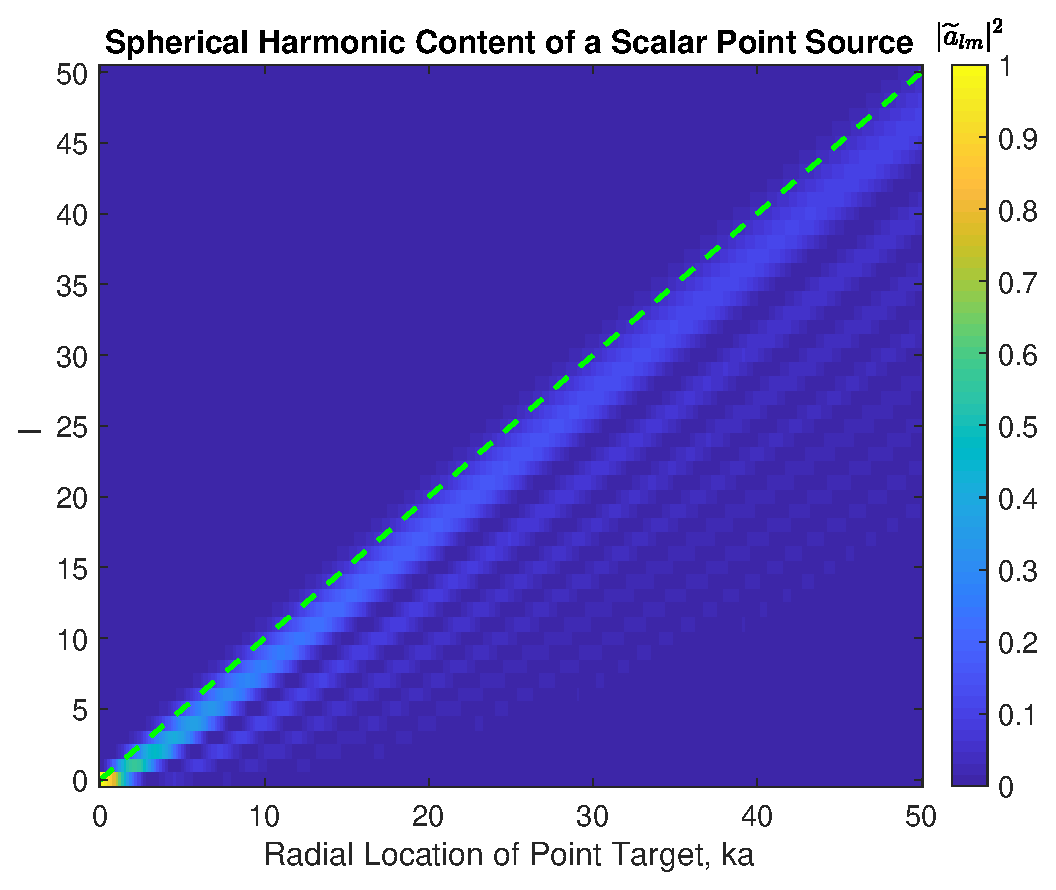
\includegraphics[width=3in]{WaveFunctions/Figures/sphharmcont}}
     \subfigure{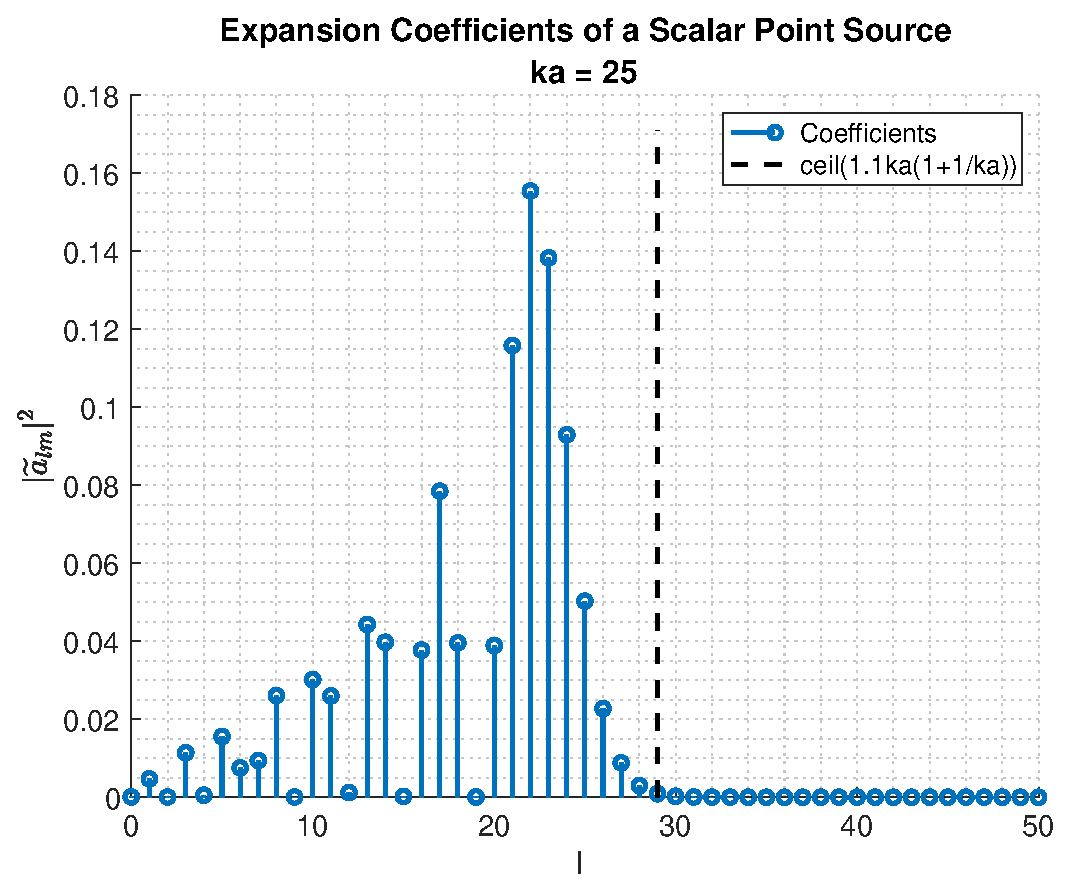
\includegraphics[width=3in]{WaveFunctions/Figures/sphharmcontex}}
  \end{tabular}
  \label{sphharmcont}
\caption{Spherical harmonic content of a scalar point source at $z = a$. Left: coefficients vs $ka$ with the line $l = ka$ plotted. Right: example of $ka = 25$ with \eqref{LLmax} plotted.}
\end{figure}










